\documentclass[conference]{IEEEtran}
\IEEEoverridecommandlockouts
% The preceding line is only needed to identify funding in the first footnote. If that is unneeded, please comment it out.
\usepackage{cite}
\usepackage{amsmath,amssymb,amsfonts}
\usepackage{algorithmic}
\usepackage{graphicx}
\usepackage{textcomp}
\usepackage{xcolor}
\usepackage{stfloats}
\usepackage{subfigure}
\def\BibTeX{{\rm B\kern-.05em{\sc i\kern-.025em b}\kern-.08em
    T\kern-.1667em\lower.7ex\hbox{E}\kern-.125emX}}
\graphicspath{ {./images/} }

\begin{document}

\title{Hypothesis: \\ A larger amount of features improves the segmentation performance\\
}

\author{\IEEEauthorblockN{Riccardo Dario Dirnberger}
\IEEEauthorblockA{\textit{Biomedical Engineering} \\
\textit{University of Bern}\\
Bern, Switzerland \\
riccardo.dirnberger@students.unibe.ch}
\and
\IEEEauthorblockN{Niklas Freudiger}
\IEEEauthorblockA{\textit{Biomedical Engineering} \\
\textit{University of Bern}\\
Bern, Switzerland \\
niklas.freudiger@students.unibe.ch}
\and
\IEEEauthorblockN{Severin Albert Willingsdorfer}
\IEEEauthorblockA{\textit{Biomedical Engineering} \\
\textit{University of Bern}\\
Bern, Switzerland \\
severin.willingsdorfer@students.unibe.ch}
}

\maketitle


%\hfill\newpage\hfill\newpage

%%% to generate tables: https://www.tablesgenerator.com/

%-----------------------------------------------------------------------------------

\begin{abstract}
%Introduction
Automated medical image analysis is nowadays common practice. Part of this process is automated image segmentation which reduces manual labour and time consumption drastically. Image segmentation relies on a set of features. Generally, the segmentation quality improves with more features, however, this also increases the time-consumption. This often-seen trade-off opens an area for further investigation. Within this study, focusing on MRI-Image brain region segmentation, the following hypothesis was examined: A larger amount of features improves the segmentation performance.

%Materials & Methods
The models were trained with various feature combinations, which included the following features: Atlas Coordinate, Intensity, Gradient-Intensity, Neighbourhood, and Noise (Gaussian and Salt \& Pepper). The models were evaluated based on the segmentation quality with metrics such as Dice score, weighted Dice score and Hausdorff-Distance. Additionally, the robustness of each model was evaluated with testing datasets with different noise types and noise levels.

%Results, Discussion, Conclusion
The most important feature is the Intensity-Feature, followed by Neighbourhood and Gradient-Intensity. The highest Dice score was achieved by combining these three features for T1-weighted images only. The combination of all three features for T1-weighted and T2-weighted did not further improve the segmentation quality but doubled the time consumption. Considering the time consumption, the model with Intensity-Feature for T1-weighted images is a good compromise as it is substantially faster with only a slight reduction in segmentation quality. Therefore, the performance concerning segmentation quality and time consumption does not improve with more features.
\end{abstract}

\begin{IEEEkeywords}
random forest, Intensity feature, Gradient-Intensity feature, Neighbourhood feature, Dice, weighted Dice
\end{IEEEkeywords}

%-----------------------------------------------------------------------------------

\section{Introduction} \label{sec:Introduction}
Medical image segmentation is a critical component within the medical image analysis pipeline and the foundation for accurate diagnosis and treatment planning. Whenever possible automatic segmentation is employed because manual segmentation is a time-consuming and expensive task. Although automated segmentation reduces the time and effort involved, the process itself can still be improved. Image segmentation uses a set of features. Even though more features can enhance segmentation accuracy, they also increase the required time. Hence, it is crucial to only choose the features with the most significant impact on segmentation accuracy for each specific problem. This way the time consumption of automatic image segmentation is minimised. This project compares and ranks features for brain region segmentation in relation to their importance for segmentation performance. It provides a guide to effective feature selection and aims to minimise the trade-off between time consumption and segmentation accuracy. \cite{Intro}

%-----------------------------------------------------------------------------------

\section{Materials \& Methods} \label{sec:Materials \& Methods}
\subsection{MRI Data} \label{subsec:MRI Data}
The 3 Tesla MRI dataset comprises 30 unrelated healthy subjects from the Human Connectome Project (HCP) dataset. Each subject has one T1-weighted and one T2-weighted image, which are not skull-stripped but are defaced for anonymisation purposes. The images have also undergone bias field correction. Additionally, the brain mask, the ground truth labels (generated by FreeSurfer 5.3), and an affine transformation for image to atlas alignment are available per subject \cite{MIA Doc}. The data of 20 of the subjects was used for training and the remaining data of 10 of the subjects for testing.

\subsection{MIA Pipeline} \label{subsec:MIA Pipeline}
The medical image analysis (MIA) pipeline comprises several steps as illustrated in Fig.~\ref{fig:MIA pipeline}. The basic pipeline was provided by our lecturers, and we made modifications to certain steps \cite{MIA Repo}. In steps 1 and 3 certain parameters were fixed at the beginning, but otherwise not modified. The main pipeline modifications were made in steps 2 and 3. Within the following a brief description of each MIA pipeline step is given:

\begin{itemize}
    \item Registration: The registration is applied to the image given an atlas image and a transformation.
    \item Preprocessing: Within the preprocessing skull-stripping and z-score normalisation is applied to the image.
    \item Feature Extraction: A variety of different image features were introduced which can be combined to different feature combinations. A more in depth description is given in subsection~\ref{subsec:Feature Extraction}.
    \item Classification: A Random Forest Classifier is used. The hyper-parameters were manually optimised to a certain extent (good Dice score with acceptable time consumption) at the project start and thereafter fixed (estimators~=~10, depth~=~30). Additionally, the random seed of NumPy was fixed to 42 to attain reproducibility.
    \item Postprocessing: As there is no actual postprocessing implemented in the given MIA pipeline, the implemented framework was removed to increase performance.
    \item Evaluation: For the evaluation a variety of testing datasets were used to calculate different metrics. An in-depth description can be found in subsection \ref{subsec:Evaluation}.
\end{itemize}

\begin{figure}[h!]
  \centering
  \includegraphics[width=0.95\linewidth]{images/MIA Pipeline.png}
  \caption{MIA Pipeline}
  \label{fig:MIA pipeline}
\end{figure}

\subsection{Feature Extraction} \label{subsec:Feature Extraction}
For the feature extraction, five features were used as shown in Fig.~\ref{subfig:features}. The Atlas-Coordinate-Feature~(C) is the base feature and must always be activated. The three main features, Intensity (I), Gradient-Intensity (G), and Neighbourhood (NH), can be used for T1-weighted (T1w) and T2-weighted (T2w) images either individually or in combination. The first two are the pixel values and the gradient of the pixel values. The Neighbourhood-Feature is a vector consisting of 15 first-order texture features~(FOTF) including mean, variance, min, and max. The FTOF is calculated over the whole image for a kernel size of 3x3. The last feature is the Noise-Feature~(GA~\&~SP). It is similar to the Intensity-Feature, however, it represents the pixel values with added noise. The feature is implemented separately for Gaussian-Noise~(GA) and Salt \& Pepper-Noise~(SP) but was always used in combination. The following parameters were used: GA (standard deviation = 500), and SP (probability = 0.02).

\begin{figure}[h!]
    \centering
    \subfigure[Features]
    {
        \includegraphics[width=0.45\linewidth, trim={0 8mm 70mm 10mm}, clip]{images/Feature Combinations.png}
        \label{subfig:features}
    }
    \hfill
    \subfigure[Feature Combinations]
    {
        \includegraphics[width=0.4\linewidth, trim={80mm 0 0 10mm}, clip]{images/Feature Combinations.png}
        \label{subfig:feature combinations}
    }
    \caption{(a) Individual features for T1-weighted (T1w) and T2-weighted (T2w) images. (b) Feature combinations from the individual features in (a).}
    \label{fig:Features and Feature Combinations}
\end{figure}

Out of these features a total of 13 feature combinations, as shown in Fig.~\ref{subfig:feature combinations}, were evaluated for segmentation performance. The Atlas-Coordinate-Feature is used as the baseline. The main features, Intensity, Gradient-Intensity, and Neighbourhood, are used individually and combined, for only T1w and only T2w, respectively. An additional combination is the fusion of the main features for T1w and T2w. The last three combinations are the main features individually with the addition of the Noise-Feature.

\subsection{Evaluation} \label{subsec:Evaluation}
The training of all feature combinations was performed on UBELIX, a high-performance computer system of the University of Bern. Each task was submitted with the following parameters: 20~CPUs, multi-core-processing, and 16~GByte of memory.

To evaluate the segmentation quality of the different combinations, the Dice score, Hausdorff-Distance (95th percentile) and weighted Dice score were calculated. The Dice score (Eq.~\ref{eq:DSC}) measures the similarity between two datasets, namely the segmentation result and ground truth segmentation. The Hausdorff-Distance (Eq.~\ref{eq:HDFDST}) is the greatest distance between the borders of the segmentation result and the ground truth segmentation. These two metrics are common tools for evaluating segmentation quality.

\begin{equation} \label{eq:DSC}
    DSC = \frac{2 \cdot |SEG \cap GT|}{|SEG|+|GT|}
\end{equation}

\begin{equation} \label{eq:HDFDST}
    d_H(SEG,GT) = max(d_{SEG,GT},d_{GT,SEG})
\end{equation}

It is important to note that the Dice score can be biased if the segmented labels differ significantly in volume. More explicitly, for labels with small volume, the Dice drops significantly, if only a few voxels are mislabelled, while for labels with large volume, the Dice remains relatively similar. To address this issue, a weighted Dice score (Eq.~\ref{eq:weightedDSC}) was introduced. This metric calculates the Dice score for each subject with respect to the volume of each label.

\begin{equation} \label{eq:weightedDSC}
weighted\ Dice = \frac{\sum_{n}^{labels} \frac{Dice_n}{volume_n}}{\sum_{n}^{labels} \frac{1}{volume_n}}
\end{equation}

The robustness of each model was evaluated by noise augmentation of the testing dataset. Therefore, the models were not only evaluated with the original testing dataset but with an additional seven noisy testing datasets. These noisy datasets included four datasets with added Gaussian noise, with a standard deviation of 300, 1'000, 2'000, and 5'000, and three datasets with added salt and pepper noise, with a probability of 1\%, 2\%, and 5\%. The highest noise levels for both types of noise generated images which are extreme cases of noise and thus, would be redone in a clinical setting. The robustness of each label was calculated by subtracting the Dice scores of the individual noisy dataset from the original dataset and calculating the mean, maximal, and minimal value of the seven attained difference-datasets. This resulted in an effective metric for robustness comparison of different feature combination models.

%-----------------------------------------------------------------------------------

\section{Results} \label{sec:Results}

Fig.~\ref{fig:diceScore} shows the segmentation quality comparison of the different feature combinations. The boxplots represent the mean Dice scores, which have been calculated over all labels per subject, of the Dice scores and weighted Dice scores. The distribution of the Dice score is in general narrower than that of the weighted Dice score. However, the difference between the two scores is mostly consistent across all feature combinations. As a result, the normal Dice score was used for all subsequent evaluations.

The Dice score is highest for the Intensity-Feature followed by Neighbourhood and Gradient-Intensity when considering individual features, as can be inferred from Fig.~\ref{fig:diceScore}. Additionally, a slightly higher Dice score is achieved for these features with T1-weighted in comparison to T2-weighted images. The combination of these three features for only T1-weighted (T1w~I-G-NH) or only T2-weighted images (T2w~I-G-NH) further increases the Dice score, particularly for T1-weighted images. However, combining all features for both image types (T1w~T2w~I-G-NH) does not result in any further improvement in Dice score.

\begin{figure}[h!]
  \centering
  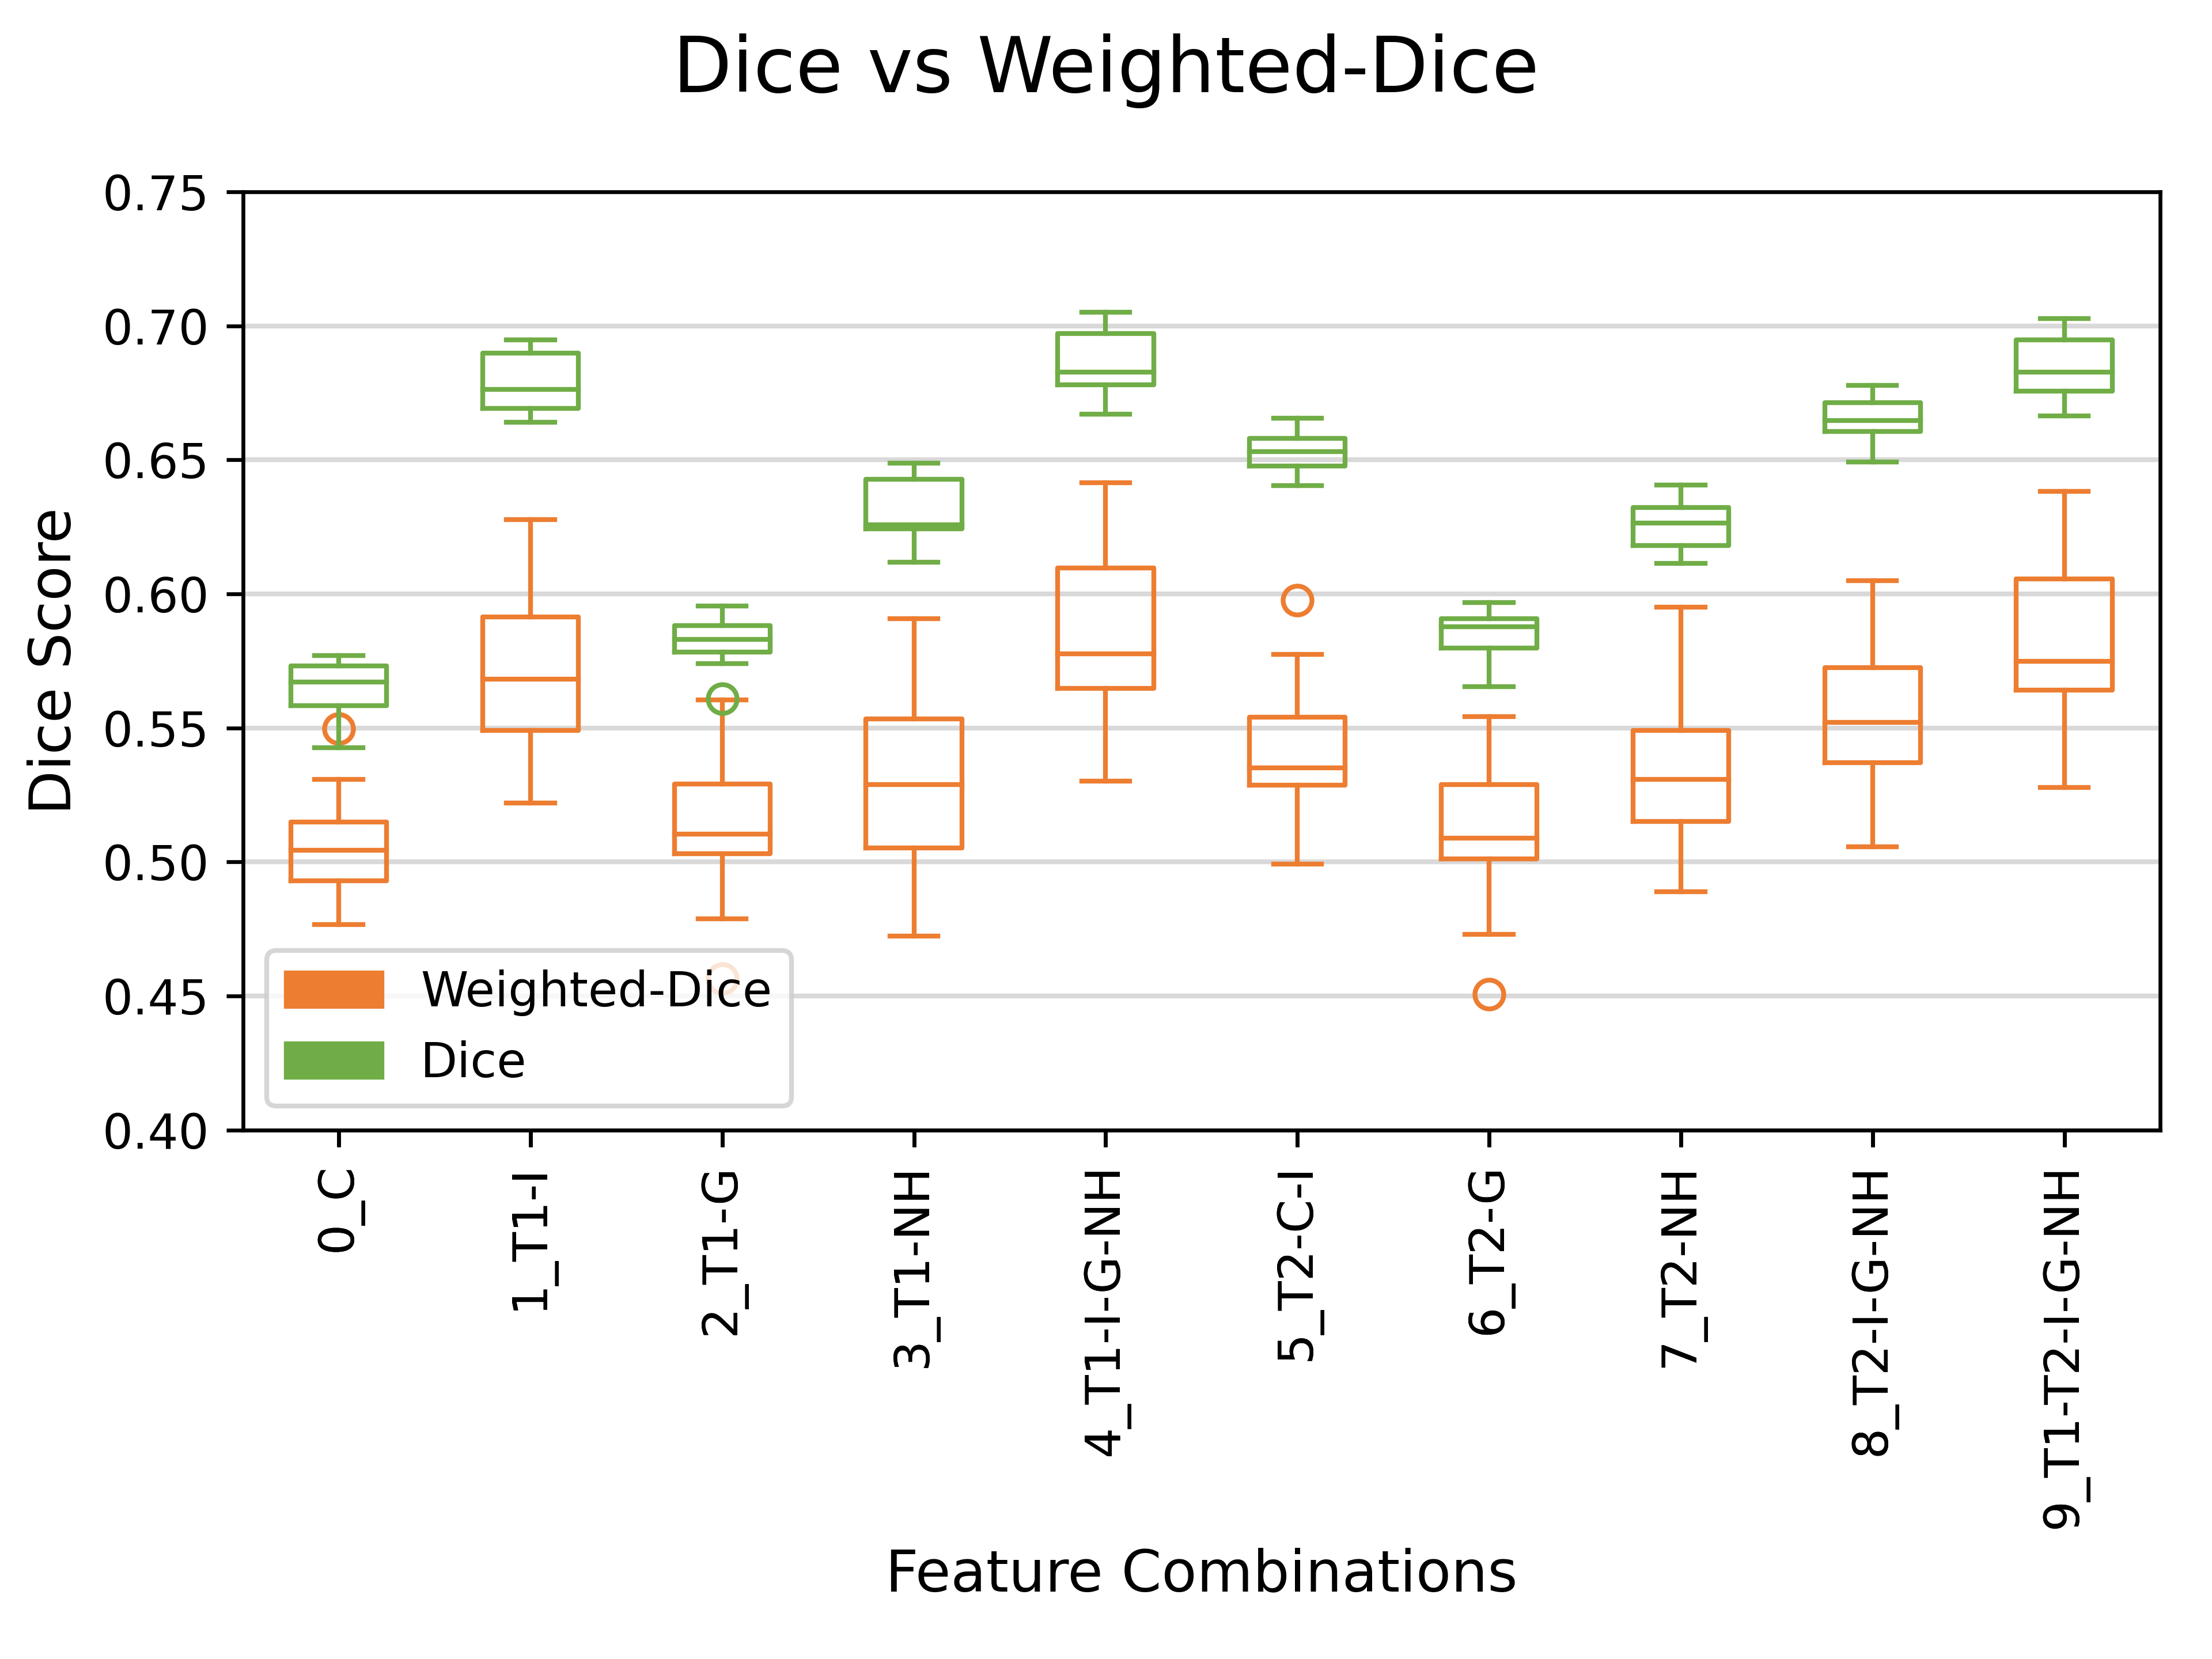
\includegraphics[width=0.95\linewidth, trim={0 4mm 0 10mm}, clip]{diceStuffZoomed}
  \caption{Comparison of Dice and weighted Dice for different feature combinations.}
  \label{fig:diceScore}
\end{figure}

The calculation of the mean over all labels causes information loss. Therefore, the results were additionally visualised for each individual label for the following feature combinations: Intensity, Gradient-Intensity, Neighbourhood, and these three combined. They are presented separated for T1-weighted and T2-weighted feature combinations in one plot in the Appendix Fig.~\ref{fig:01_T1W_C_I_and_05_T2W_C_I},~\ref{fig:02_T1W_C_G_and_06_T2W_C_G},~\ref{fig:03_T1W_C_NH_and_07_T2W_C_NH},~and~\ref{fig:04_T1W_C_I_G_NH_and_08_T2W_C_I_G_NH}. The plots reveal that there is no difference or variation to the presented results in Fig.~\ref{fig:diceScore} for these T1-weighted and T2-weighted feature combinations.

The highest Dice scores are achieved by the feature combinations numbered as 4~(T1w~I-G-NH) and 9~(T1w~T2w~I-G-NH) in Fig.~\ref{fig:diceScore}. To facilitate comparison, only these two are plotted in Fig.~\ref{fig:bestRun} for each label. The top plot displays the Dice scores as boxplots and the mean Hausdorff-Distance over all subjects as dots. The bottom plot shows the robustness, which is described by the relative Dice score, as detailed in subsection~\ref{subsec:Evaluation}. The dot represents the mean, and the bars the maximum and minimum values.

\begin{figure*}[h!]
  \centering
  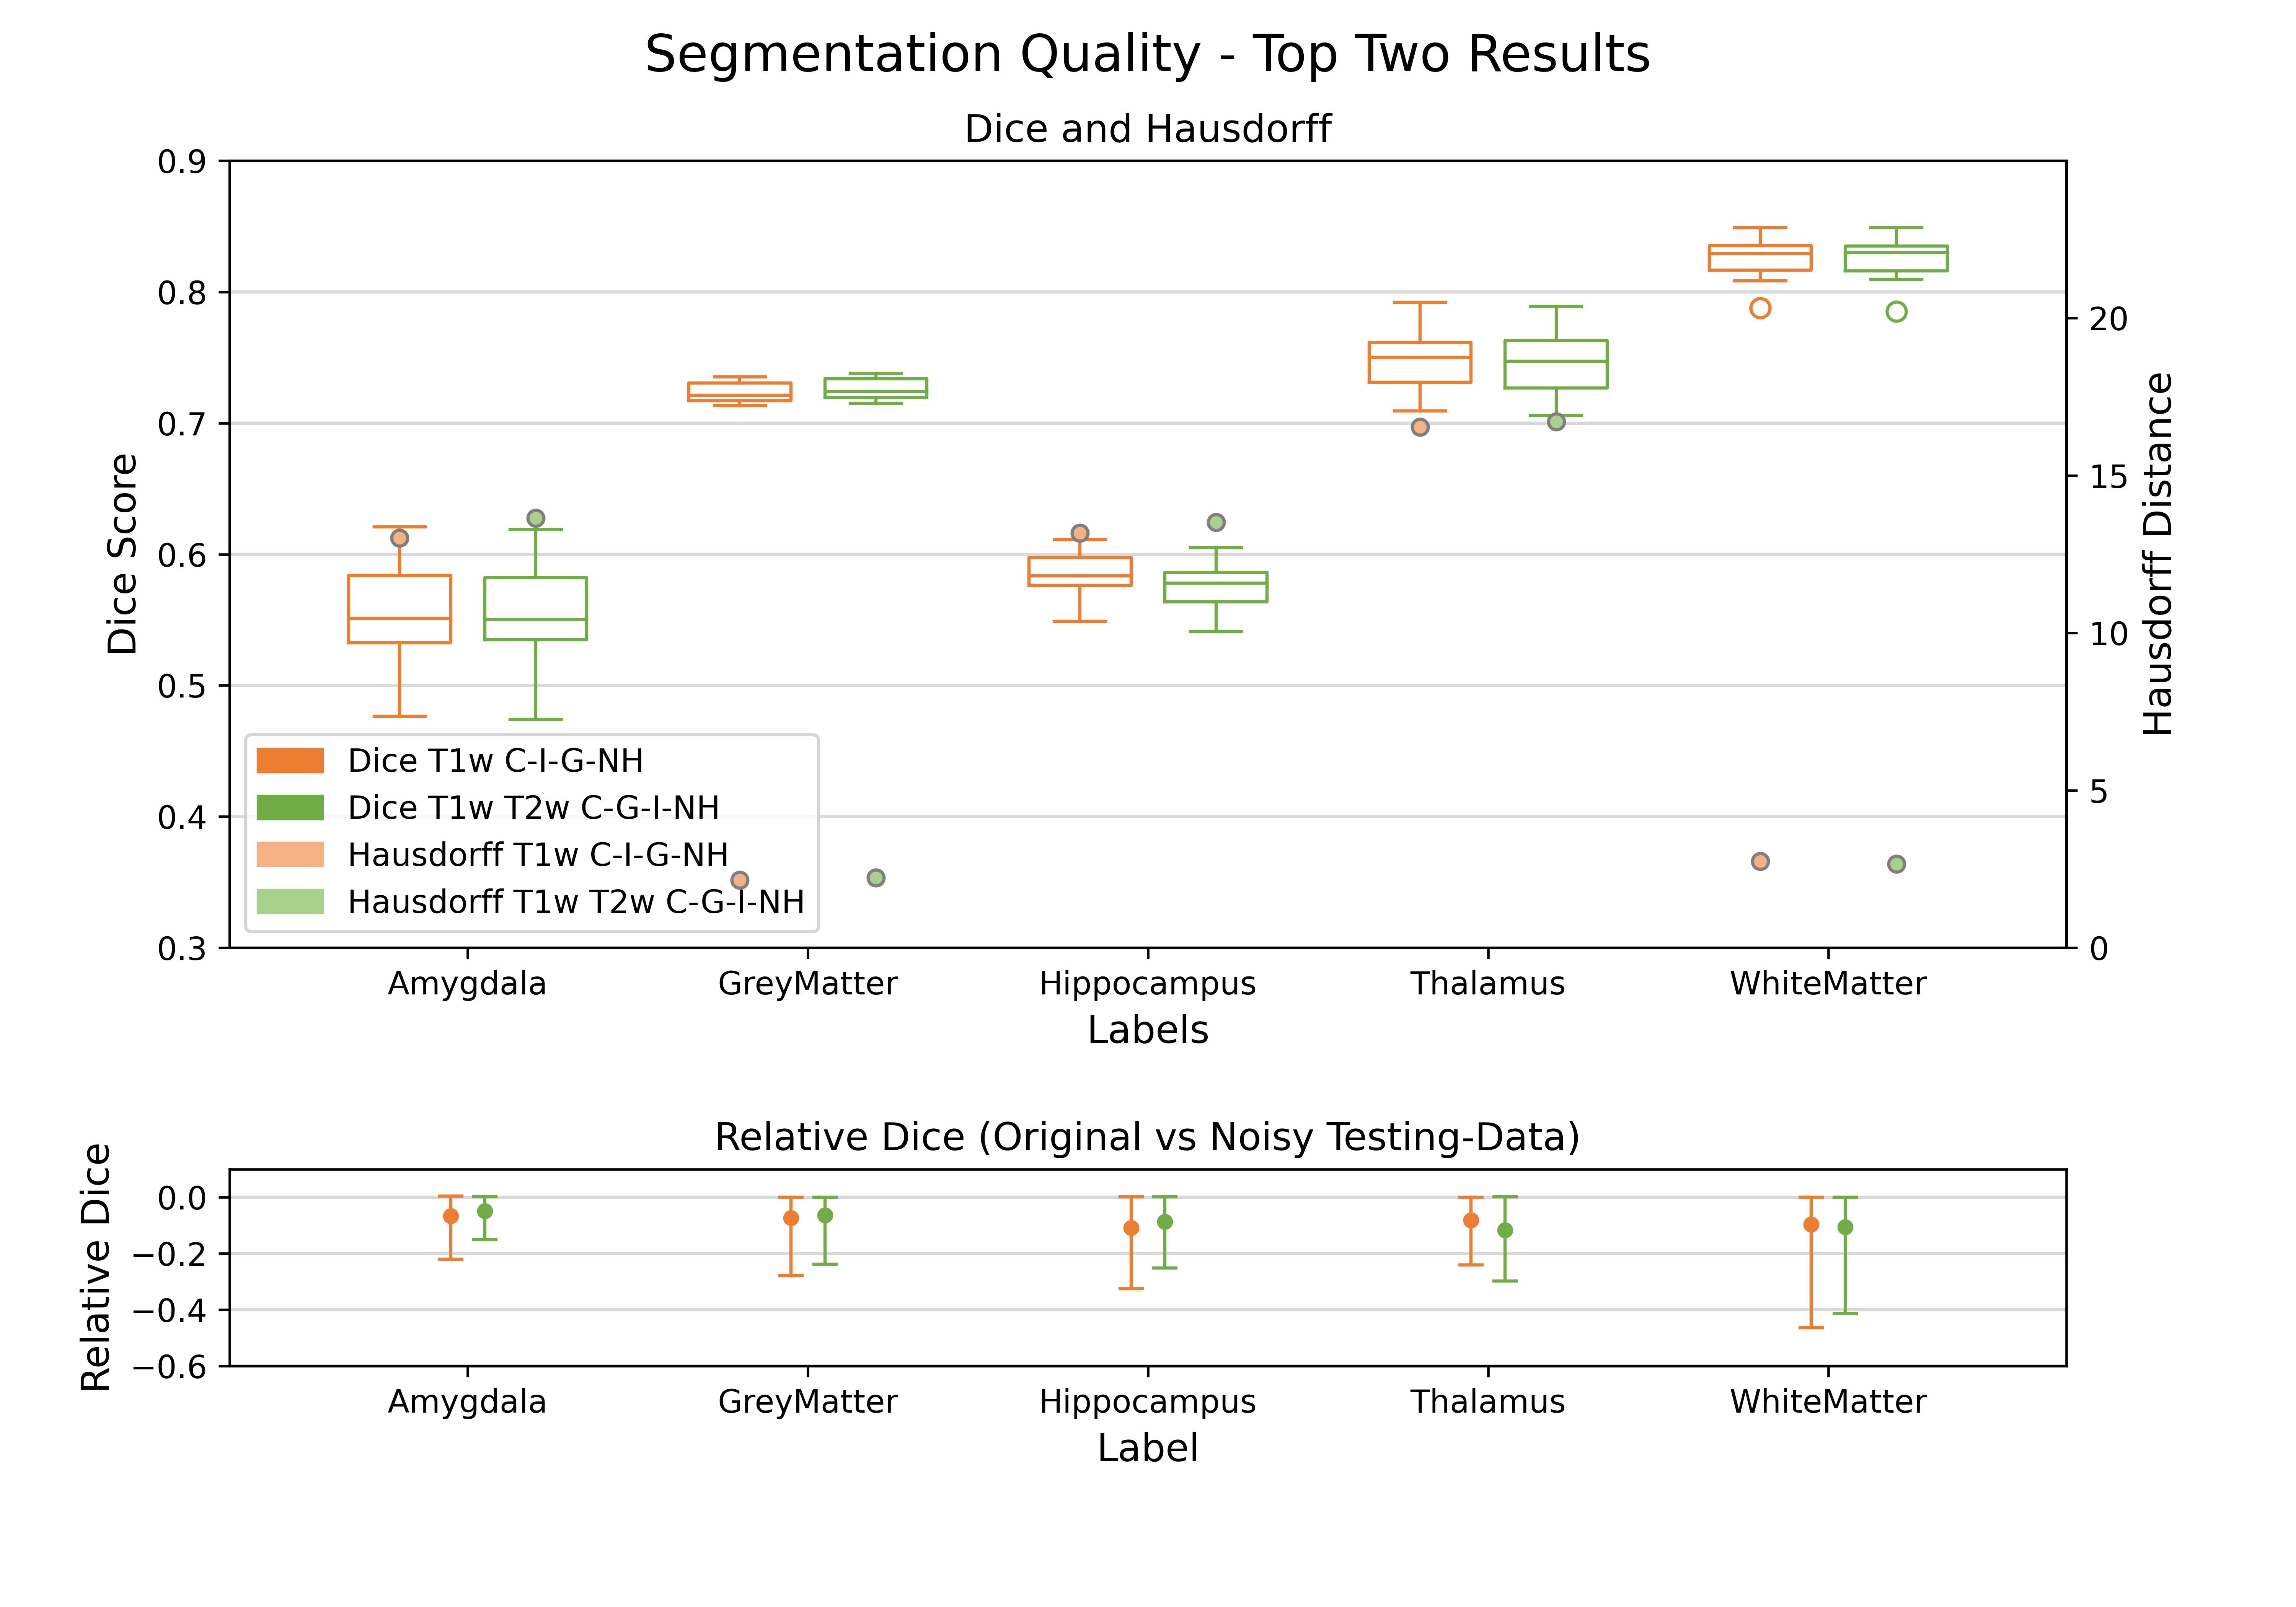
\includegraphics[width=0.8\linewidth, trim={0 8mm 0 10mm}, clip]{04_T1W_C_I_G_NH_and_09_T1W_T2W_C_I_G_NH_zoomed}
  \caption{Direct comparison of the two best feature combinations.}
  \label{fig:bestRun}
\end{figure*}

In addition to the visual comparison given in Fig.~\ref{fig:bestRun} the results are also compared numerically as median and mean values in Tab.~\ref{table:Median} and Tab.~\ref{table:Mean}, respectively. By comparing the average over all labels of the four variants, it can be concluded that the difference between the two feature combinations is negligible, as differences are only in the thousandths.

\begin{table}[h!]
    \centering
    \caption{Comparison of the two best Feature combinations according to median Dice score for all labels.}
    \label{table:Median}
    \begin{IEEEeqnarraybox}[\IEEEeqnarraystrutmode\IEEEeqnarraystrutsizeadd{2pt}{0pt}]{x/r/Vx/r/v/r/x}
        \IEEEeqnarraydblrulerowcut\\
        &Median             &&& T1w\ C\text{-}I\text{-}G\text{-}NH  && T1w\ T2w\ C\text{-}I\text{-}G\text{-}NH  &\\
        \IEEEeqnarraystrutsize{0pt}{0pt}\\
        \IEEEeqnarraydblrulerowcut\\
        &Amygdala           &&& 0.5511                              && 0.5502                                   &\\
        &Grey Matter        &&& 0.7212                              && 0.7241                                   &\\
        &Hippocampus        &&& 0.5834                              && 0.5781                                   &\\
        &Thalamus           &&& 0.7500                              && 0.7473                                   &\\
        &White Matter       &&& 0.8292                              && 0.8299                                   &\\
        &                   &&&                                     &&                                          &\\
        &\textbf{Average}   &&& \textbf{0.6870}                     &&\textbf{0.6859}                           &\\
        \IEEEeqnarraydblrulerowcut\\
        &\IEEEeqnarraymulticol{7}{s}{}%
    \end{IEEEeqnarraybox}
\end{table}

\begin{table}[h!]
    \centering
    \caption{Comparison of the two best Feature combinations according to mean Dice score for all labels.}
    \label{table:Mean}
    \begin{IEEEeqnarraybox}[\IEEEeqnarraystrutmode\IEEEeqnarraystrutsizeadd{2pt}{0pt}]{x/r/Vx/r/v/r/x}
        \IEEEeqnarraydblrulerowcut\\
        &Mean               &&& T1w\ C\text{-}I\text{-}G\text{-}NH  && T1w\ T2w\ C\text{-}I\text{-}G\text{-}NH &\\
        \IEEEeqnarraystrutsize{0pt}{0pt}\\
        \IEEEeqnarraydblrulerowcut\\
        &Amygdala           &&& 0.5523                              && 0.5518                                   &\\
        &Grey Matter        &&& 0.7234                              && 0.7263                                   &\\
        &Hippocampus        &&& 0.5844                              && 0.5767                                   &\\
        &Thalamus           &&& 0.7468                              && 0.7454                                   &\\
        &White Matter       &&& 0.8252                              && 0.8251                                   &\\
        &                   &&&                                     &&                                          &\\
        &\textbf{Average}   &&& \textbf{0.6864}                     && \textbf{0.6851}                          &\\
        \IEEEeqnarraydblrulerowcut\\
        &\IEEEeqnarraymulticol{7}{s}{}%
    \end{IEEEeqnarraybox}
\end{table}

%-----------------------------------------------------------------------------------

\section{Discussion \& Conclusion} \label{sec:Discussion \& Conclusion}
Some features have a more significant impact on the segmentation quality than others as evident in Fig.~\ref{fig:diceScore}. Among the individual features, the Intensity-Feature has the most significant impact. This is to be expected as the grey value of a pixel in an MRI image represents the water content of the tissue. Therefore, a narrow range of pixel intensities corresponds to a specific tissue type, which is associated with a label.

Fig.~\ref{fig:bestRun} shows, that the segmentation quality of grey and white matter are the best when considering the Dice score and the Hausdorff-Distance. Both labels have a high Dice score with a narrow distribution, and the Hausdorff-Distances are the lowest. This indicates a high similarity and good accuracy between the segmentation result and the ground truth. These results can be expected for labels with a large volume. However, labels with a smaller volume, such as the amygdala and the hippocampus, show a reduced Dice score with an about five times higher Hausdorff-Distance. This indicates a lower similarity and a reduced accuracy. On the other hand, the results for the thalamus do not match these observations. The thalamus has a small volume, much smaller than grey and white matter, but about twice the size of the hippocampus. Nonetheless, the Dice scores lie between those of grey and white matter, indicating a good segmentation to ground truth similarity. However, the Hausdorff-Distance is even larger than for the other two small labels, indicating an even lower accuracy.

Further can be observed that in four out of five labels, the Dice score is slightly higher, and the Hausdorff-Distance smaller for the T1w~C-I-G-NH feature combination compared to the T1w~T2w~C-I-G-NH feature combination. This visual indication is supported numerically by the averages in Tab.~\ref{table:Median} and Tab.~\ref{table:Mean}. However, the latter outperforms the first in robustness in four labels. Therefore, it can be deduced that T1-weighted images improve segmentation quality whereas the addition of T2-weighted images slightly reduces it, but with the added benefit of increased robustness.

The last three feature combinations in Fig.~\ref{fig:Features and Feature Combinations} show the results for training with added noisy images. However, this did not lead to the expected improvement in robustness. One possible explanation for this is that only one specific noise level was implemented for both Gaussian and salt and pepper noise.

Regarding the hypothesis, the segmentation performance may not only be characterised by the quality of segmentation but also by the time taken to train and evaluate a model. In our runs on UBELIX, we found that the two best-performing models (T1w~C-I-G-NH and T1w~T2w~C-I-G-NH), which achieved similar segmentation quality, had a considerable difference in runtime. The latter took 26 hours, which is about twice as long as the former. If a slightly lower segmentation quality is sufficient for the respective task the runtime can be further reduced. For example, the third best model (T1w~C-I) had a runtime of only about 30 minutes. Therefore, more features do not necessarily increase the segmentation performance, especially if not the absolute best segmentation quality is required for the respective task the runtime can be substantially reduced by removing features.

As a final remark, the outcome may differ for other constant parameters, particularly for hyper-parameters related to the random forest classifier. However, changing the fixed NumPy seed is expected to have minimal impact.

%-----------------------------------------------------------------------------------

%\section{References}
\begin{thebibliography}{00}

\bibitem{Intro} Giger M., Zheng Y., Gloecker J., Studer A., Comaniciu D., Davatzikos C. (2008). "Selective fusion of features for accurate brain image segmentation using k-nearest neighbor classifier". NeuroImage, 41(3):1140-1152. DOI: 10.1016/j.neuroimage.2008.03.049

\bibitem{MIA Repo} "Medical Image Analysis Laboratory - Repository" [Online]. Available: https://github.com/ubern-mia/MIALab

\bibitem{MIA Doc} "Medical Image Analysis Laboratory - Documentation" [Online]. Available: https://mialab.readthedocs.io/en/latest


\end{thebibliography}

%-----------------------------------------------------------------------------------
\clearpage
\onecolumn 

\appendix

\begin{appendices} \label{Appendix}

\listoffigures

\listoftables

%%\listofequations

\newpage


\begin{figure*}[h!]
    \centering
    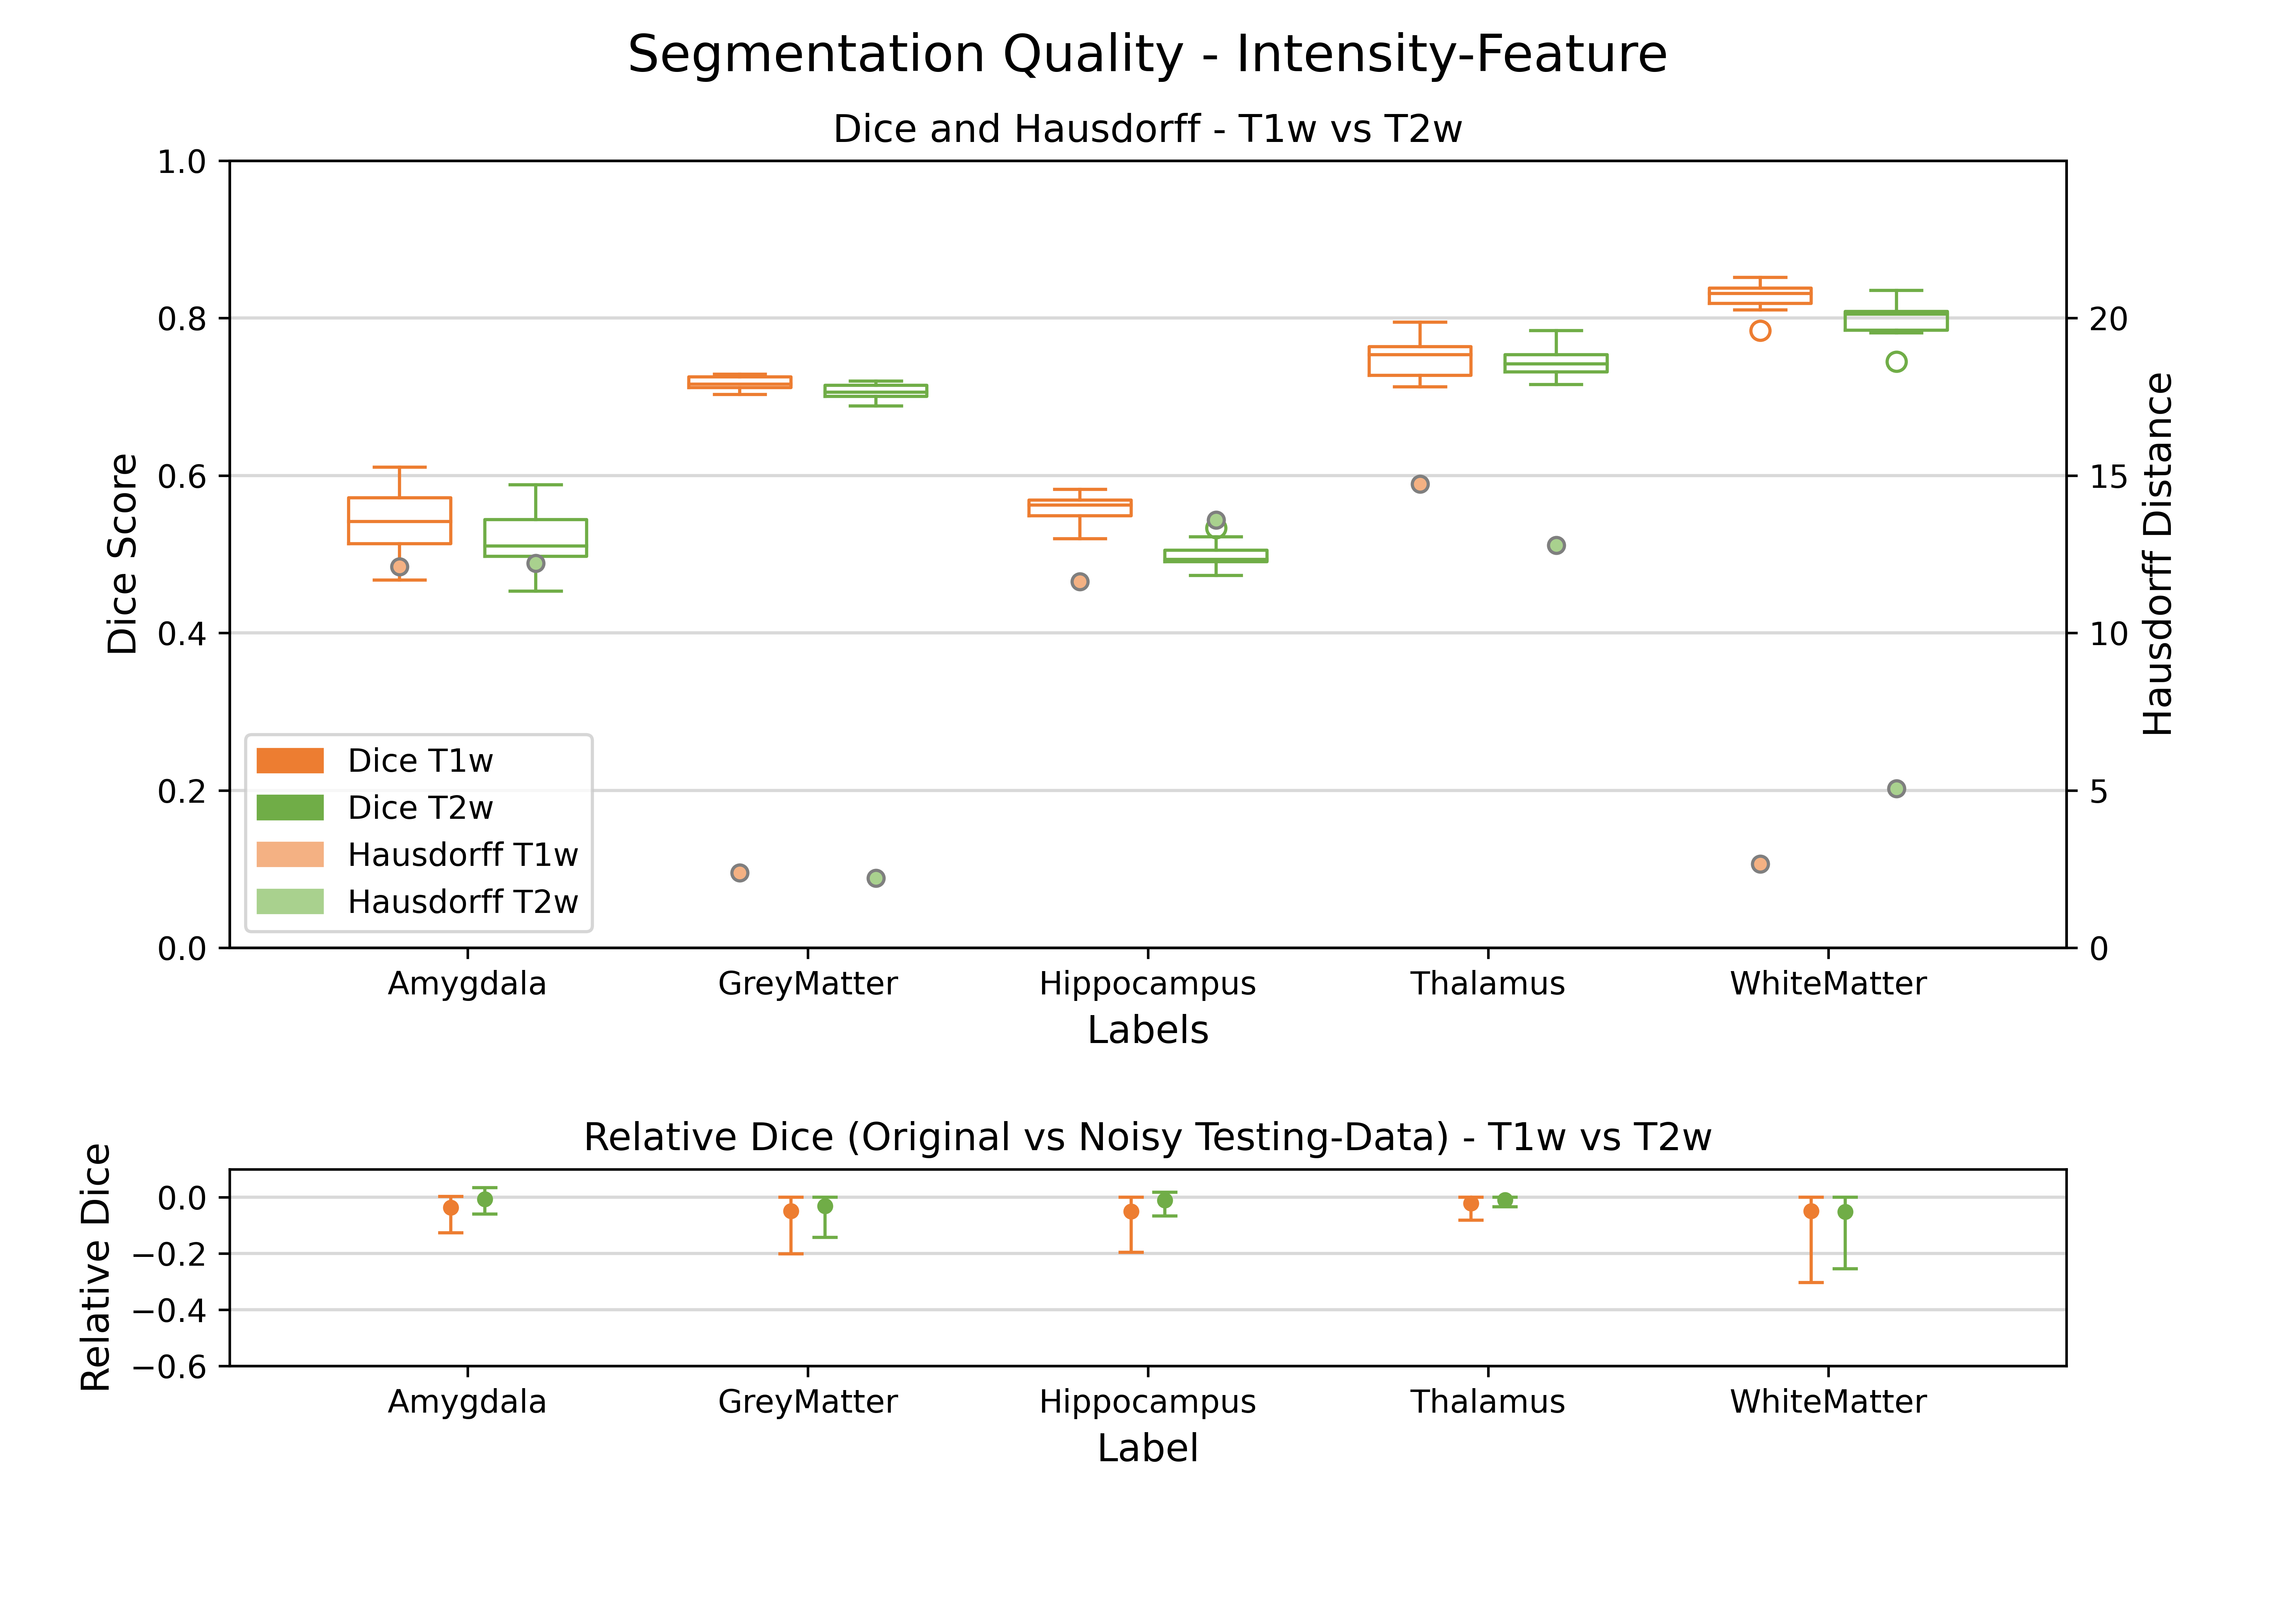
\includegraphics[width=0.9\textwidth, trim={0 15mm 0 10mm}, clip]{images/01_T1W_C_I_and_05_T2W_C_I.png}
      \caption{Comparison T1- and T2-weighted - Intensity-Feature}
    \label{fig:01_T1W_C_I_and_05_T2W_C_I}
\end{figure*}
%\hspace{100mm}
\begin{figure*}[h!]
    \centering
    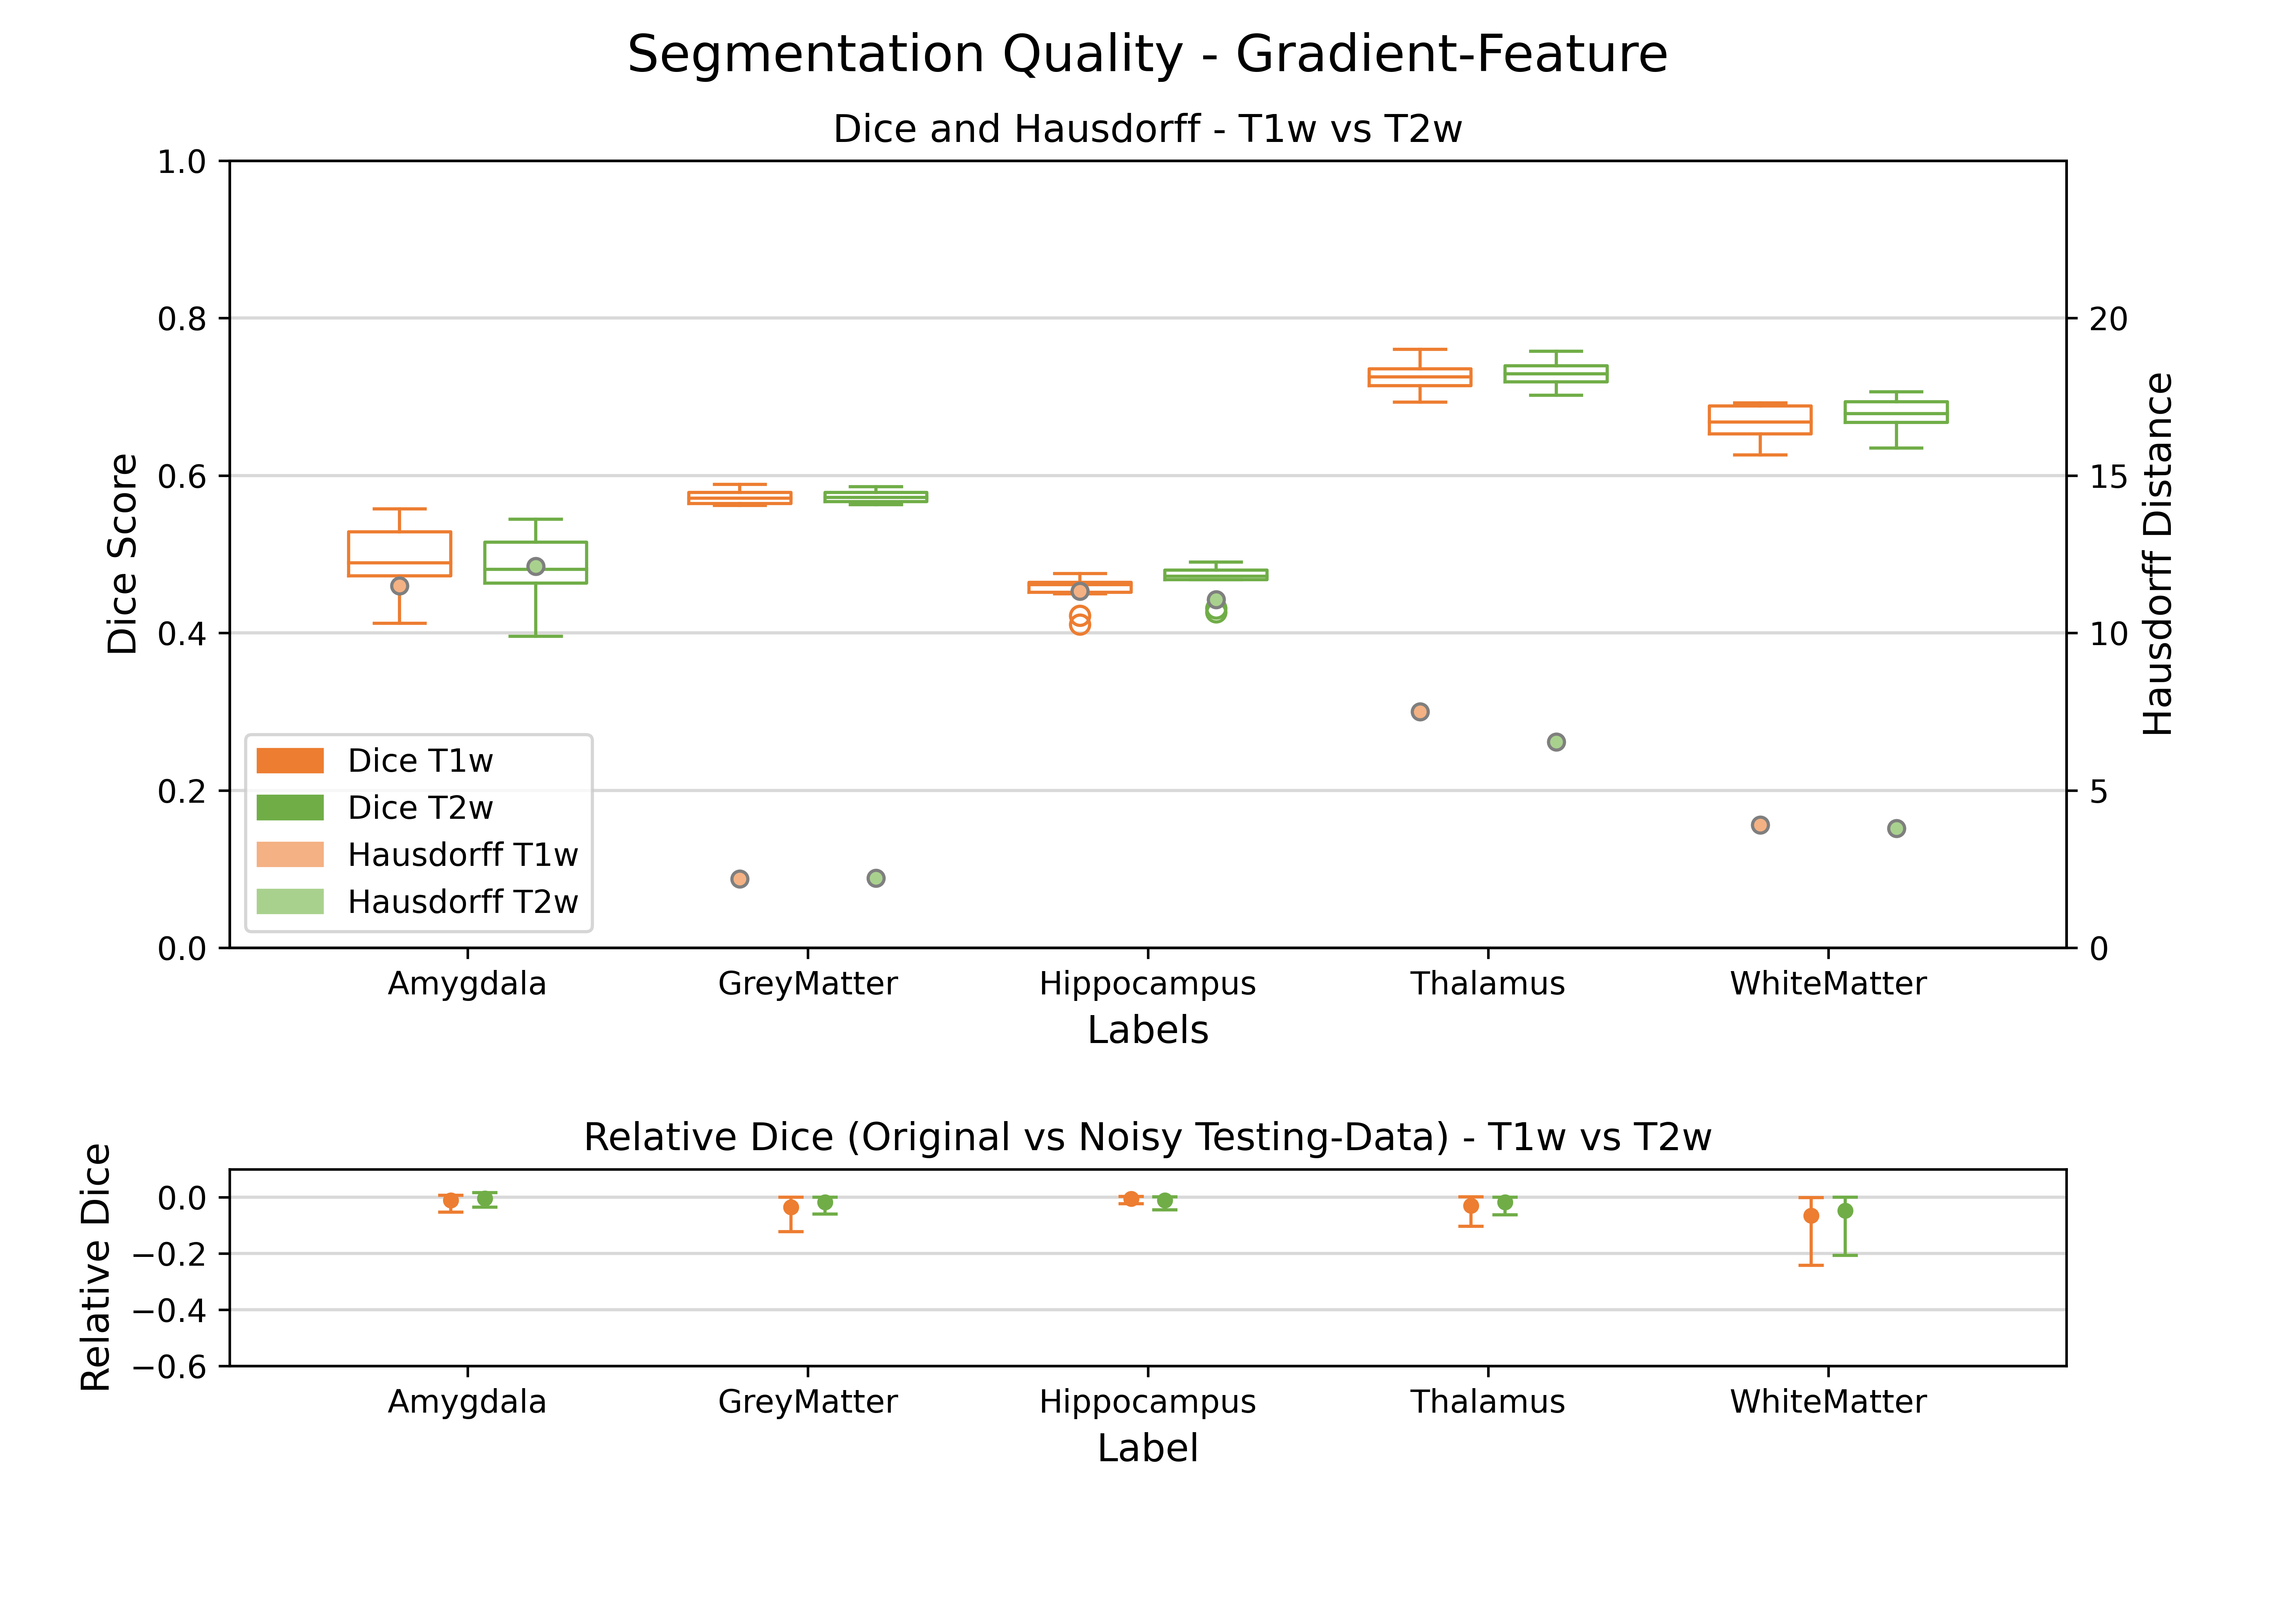
\includegraphics[width=0.9\textwidth, trim={0 15mm 0 10mm}, clip]{images/02_T1W_C_G_and_06_T2W_C_G.png}
      \caption{Comparison T1- and T2-weighted - Gradient-Intensity-Feature}
    \label{fig:02_T1W_C_G_and_06_T2W_C_G}
\end{figure*}


\begin{figure*}[h!]
    \centering
    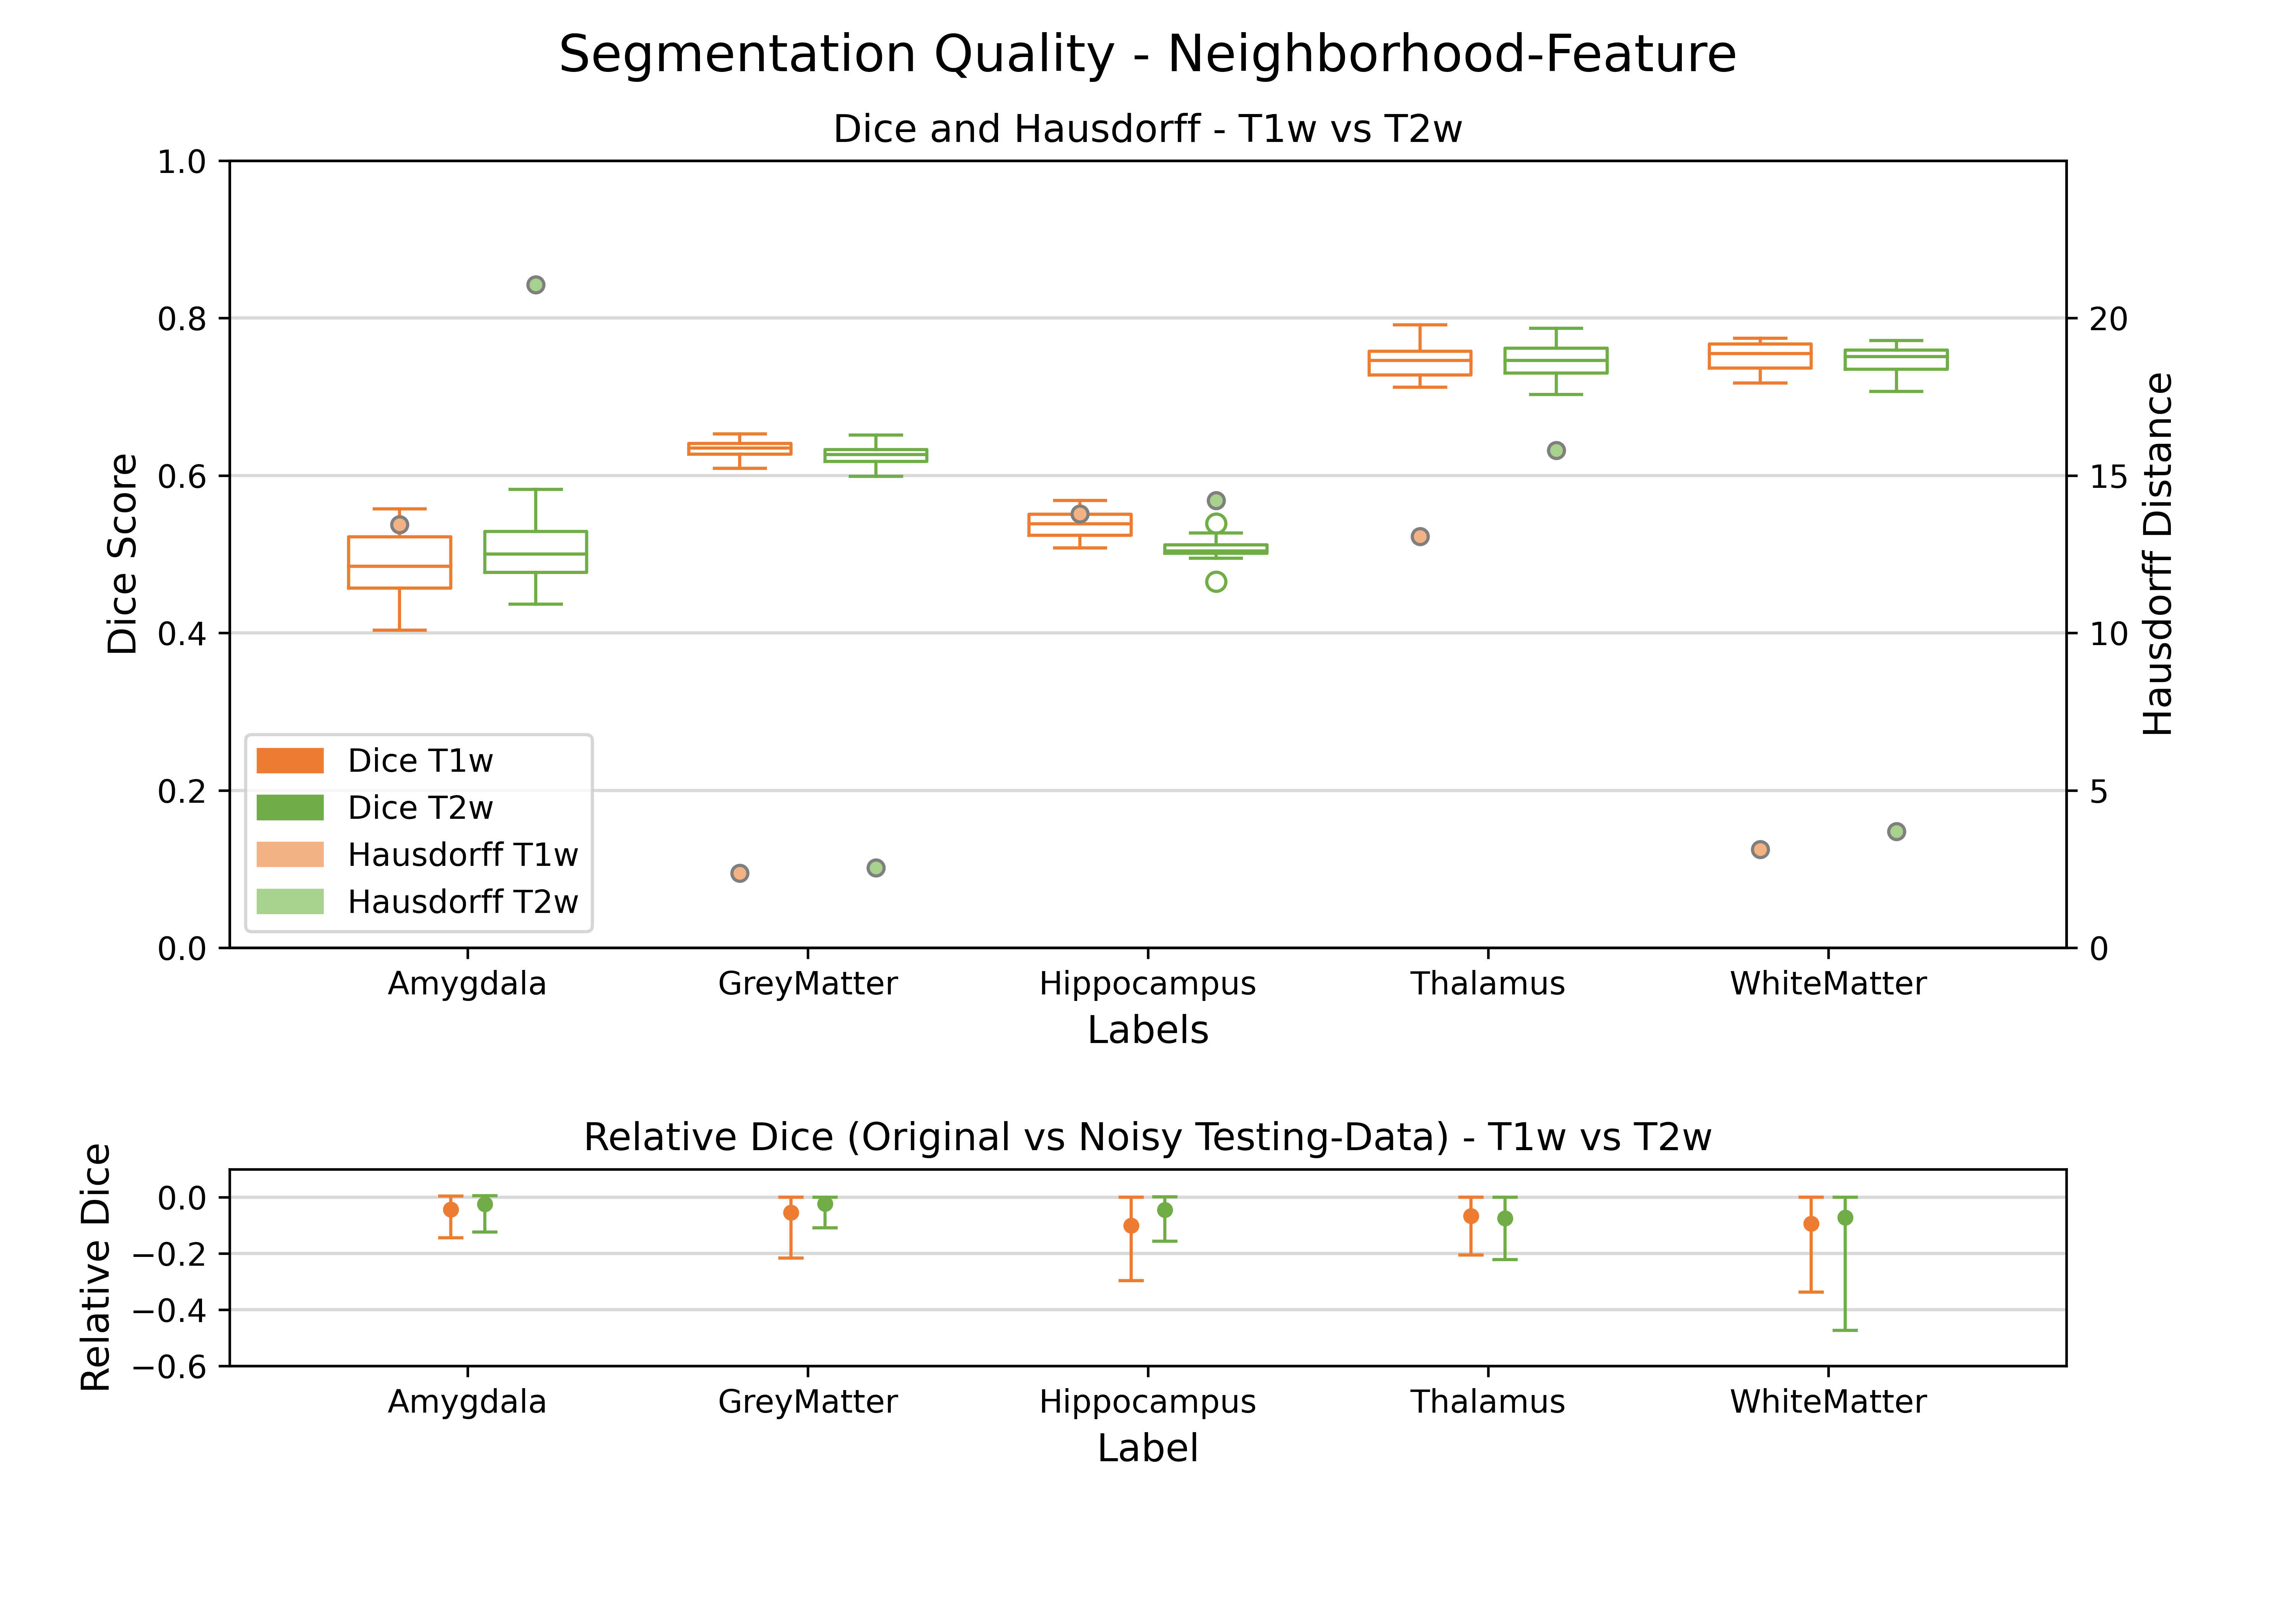
\includegraphics[width=0.9\textwidth, trim={0 15mm 0 10mm}, clip]{images/03_T1W_C_NH_and_07_T2W_C_NH.png}
    \caption{Comparison T1- and T2-weighted - Neighbourhood-Feature}
    \label{fig:03_T1W_C_NH_and_07_T2W_C_NH}
\end{figure*}
%\hspace{100mm}
\begin{figure*}[h!]
    \centering
    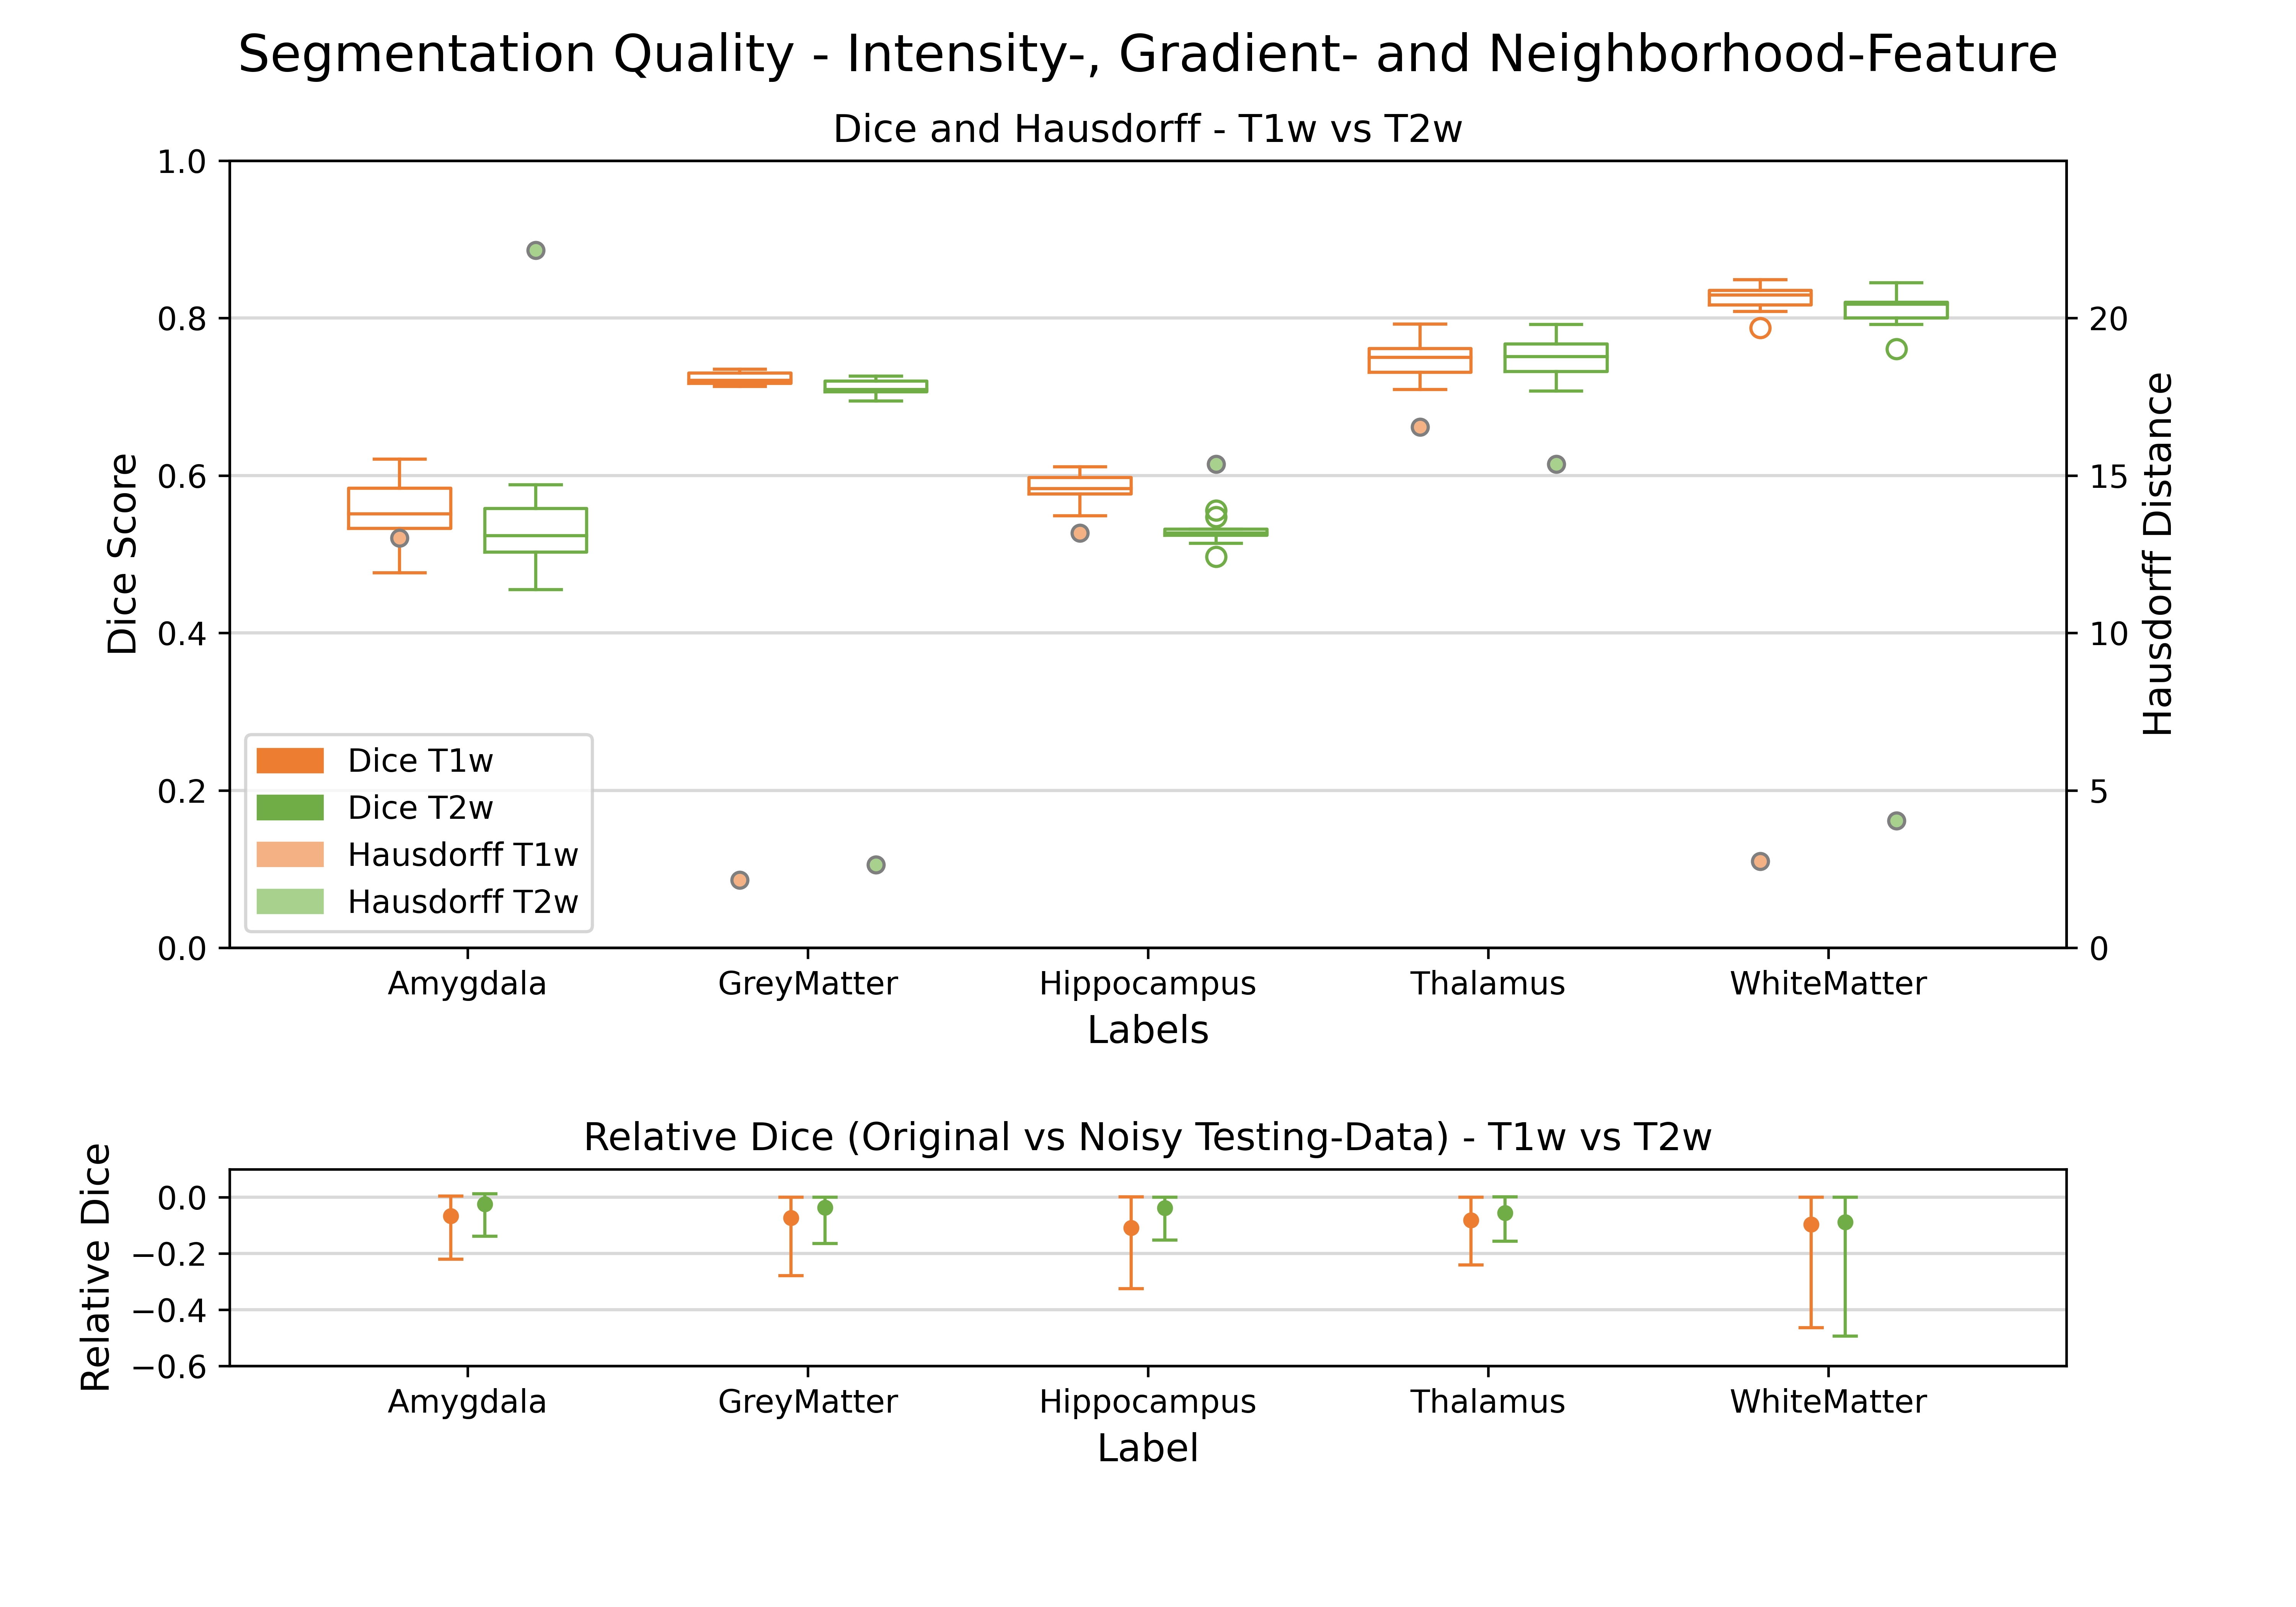
\includegraphics[width=0.9\textwidth, trim={0 15mm 0 10mm}, clip]{images/04_T1W_C_I_G_NH_and_08_T2W_C_I_G_NH.png}
    \caption{Comparison T1- and T2-weighted - Intensity-, Gradient-Intensity-, Neighbourhood-Feature}
    \label{fig:04_T1W_C_I_G_NH_and_08_T2W_C_I_G_NH}
\end{figure*}


\end{appendices}

\end{document}